% Phase 3: archived numerical results, original executed notebook, and official Codabench screenshot.
% Reproduce figures from code/phase3/analysis/figures.py; do not edit scores by hand.
\clearpage
\section{Phase 3: Sentence-Level Rhetorical Role Prediction}
\label{sec:phase3}

\subsection{Research question and task formulation}
Legal decisions contain factual narratives, petitions, statutory references, earlier decisions, reasoning and operative rulings. The same sentence may communicate evidence, an advocate's position, or a court's conclusion depending on surrounding sentences. We therefore cast rhetorical-role prediction as contextual sentence classification while preserving the order of an entire judgment. For a judgment $D=(s_1,\ldots,s_n)$ with a target sentence $s_i$ and optionally its neighboring context $C_i$, the classifier produces
\begin{equation}\label{eq:p3-task}
 p_\theta(y_i=k\mid s_i,C_i)=\operatorname{softmax}(\mathbf W h_\theta(s_i,C_i)+\mathbf b)_k,\qquad
 \hat y_i=\arg\max_{k\in\{1,\ldots,13\}}p_\theta(y_i=k\mid s_i,C_i).
\end{equation}
\begin{sloppypar}
The official label vocabulary is exactly \method{Fact}, \method{Issue}, \method{Argument\allowbreak Petitioner}, \method{Argument\allowbreak Respondent}, \method{Statute}, \method{Dissent}, \method{Precedent\allowbreak Relied\allowbreak Upon}, \method{Precedent\allowbreak Not\allowbreak Relied\allowbreak Upon}, \method{Precedent\allowbreak Overruled}, \method{Ruling\allowbreak By\allowbreak Lower\allowbreak Court}, \method{Ratio\allowbreak Of\allowbreak The\allowbreak Decision}, \method{Ruling\allowbreak By\allowbreak Present\allowbreak Court} and \method{None}. The label-to-index mapping is read directly from the supplied \path{label_vocab.json}; names and capitalizations are not rewritten. Every prediction list must have the same length as the original document's sentence list.
\end{sloppypar}

The official primary metric is macro-averaged F1 over \emph{all} 13 roles, including roles with zero development support:
\begin{equation}\label{eq:p3-f1}
\mathrm{MacroF1}=\frac1{13}\sum_{k=1}^{13}\frac{2\,\mathrm{TP}_k}{2\,\mathrm{TP}_k+\mathrm{FP}_k+\mathrm{FN}_k},\qquad 0/0:=0.
\end{equation}
Macro-precision and macro-recall are companion measures. A low-frequency label may have a large effect on Macro-F1 despite contributing few sentences. The experiment set therefore investigated four original Phase-1 architectures, multiple adaptation mechanisms, sentence context, domain-specific learning, structured label decoding, class balancing and knowledge distillation.

\subsection{Dataset and evidence integrity}
\label{sec:p3-data}
All data originate from \method{Exploration-Lab/CS-781-Capstone}, folder \method{Phase\_3\_RR}; no external pretrained language models or training corpora were used. The train/development lists each comprise document records with \method{id}, an ordered \method{text} sentence array and aligned \method{labels}; hidden-test files instead map document IDs directly to sentence arrays. This structural distinction was discovered during ingestion and handled explicitly, without changing sentence order.

\begin{table}[htbp]\centering\small
\caption{Exact Phase-3 data sizes from the completed exploratory notebook. Train/dev include labels; test labels are withheld.}
\label{tab:p3-sizes}
\begin{tabular}{@{}lrrr rrr@{}}\toprule
 & \multicolumn{3}{c}{Documents} & \multicolumn{3}{c}{Sentences}\\
Domain & Train & Dev & Test & Train & Dev & Test\\\midrule
Corporate Law (CL) & 40 & 5 & 5 & 10,593 & 1,396 & 1,339\\
Information Technology (IT) & 40 & 5 & 5 & 6,252 & 746 & 858\\
\midrule
Total & 80 & 10 & 10 & 16,845 & 2,142 & 2,197\\\bottomrule
\end{tabular}
\end{table}
The mean sentence count alone is misleading because judgments vary considerably in length: the largest training document has 1,816 sentences in CL and 442 in IT, whereas the median counts are 120.5 and 126.5 respectively. Document-level leakage matters: the notebook checked 100 documents across train/dev/test and found no exact normalized-text duplicate across different splits, no overlapping domain IDs and no blank sentences. These are \emph{exact-match} integrity checks, not exhaustive near-duplicate detection.

\begin{figure}[htbp]\centering
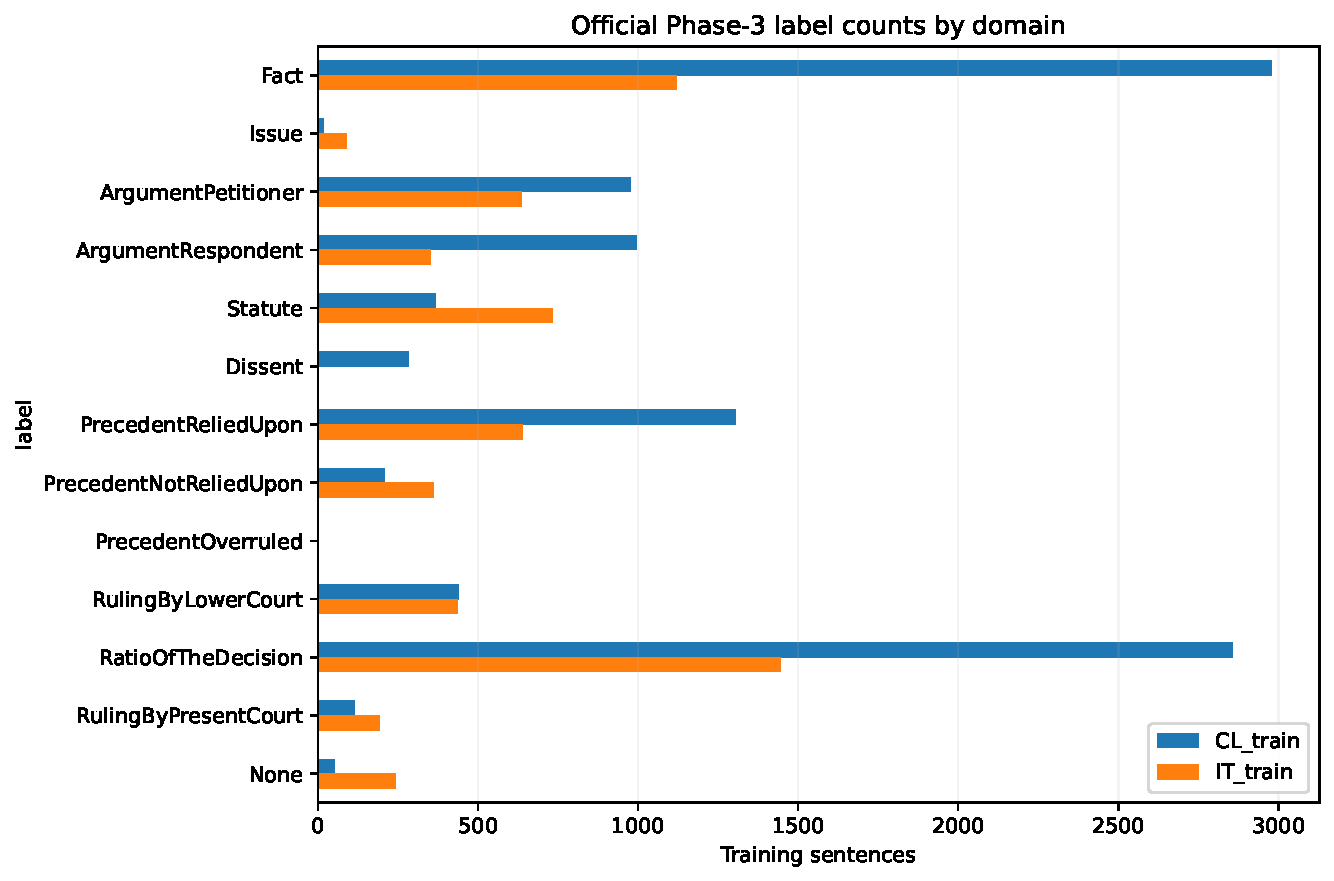
\includegraphics[width=.86\linewidth]{figures/phase3/p3_label_distribution.pdf}
\caption{Training-role distribution by legal domain, based on the official label counts recorded in the notebook. Both domains are imbalanced and differ substantially in the use of certain roles.}
\label{fig:p3-labels}
\end{figure}
\method{Fact} appears 2,979 times in CL training but 1,119 times in IT; \method{Ratio\allowbreak Of\allowbreak The\allowbreak Decision} appears 2,856 and 1,445 times. The rare \method{Precedent\allowbreak Overruled} occurs only three times in IT training and zero times in CL; \method{Dissent} occurs 284 times in CL training and zero times in IT. \method{Issue} appears 17 times in CL and 90 times in IT. Consequently, class weighting cannot solve all low-support errors: in particular, no method can infer an absent class from same-domain supervised examples alone. There are 0 examples of both \method{Dissent} and \method{Precedent\allowbreak Overruled} in the 2,142-sentence development set, so their reported per-class F1 scores are zero by the explicit 13-label convention.

\subsection{Tokenization, sentence representation and truncation}
\label{sec:p3-preprocess}
The original Phase-1 legal byte-level BPE tokenizer was recovered as \path{legal_bpe_32k.json} (32,000 entries; pad, BOS, EOS and UNK IDs $0,1,2,3$). No new BPE was fit for this phase. Sentences were tokenized without automatic specials, then packed as BOS + content + EOS. The pooled training-token distribution had its 95th percentile below 128, so the notebook fixed its maximum input length to 128 BPE tokens. The observed fraction of single-sentence training inputs beyond 128 tokens was 1.38\% for CL and 2.85\% for IT. Overlong sentences were shortened by keeping 75\% of the available budget from the beginning and 25\% from the end. This preserves some late conclusions but can remove legally salient clauses in the middle; it is an explicit information-loss limitation.

For the causal decoders, the 768-dimensional hidden representation at the \emph{last non-padding EOS position} is used for classification. Causal masking makes right padding invisible to that location. The Prefix-LM variant was run with full-sentence bidirectional attention and an explicit key-padding mask. The encoder--decoder variant used only the pretrained encoder, with its own padding-safe attention, not the pretrained cross-attentive decoder. These architectural distinctions matter: transferring the encoder only is not a direct measure of the usefulness of the model's pretrained decoder or the original sequence-to-sequence generation objective. The 13-class head is a dropout layer followed by a linear projection.

\begin{figure}[htbp]\centering
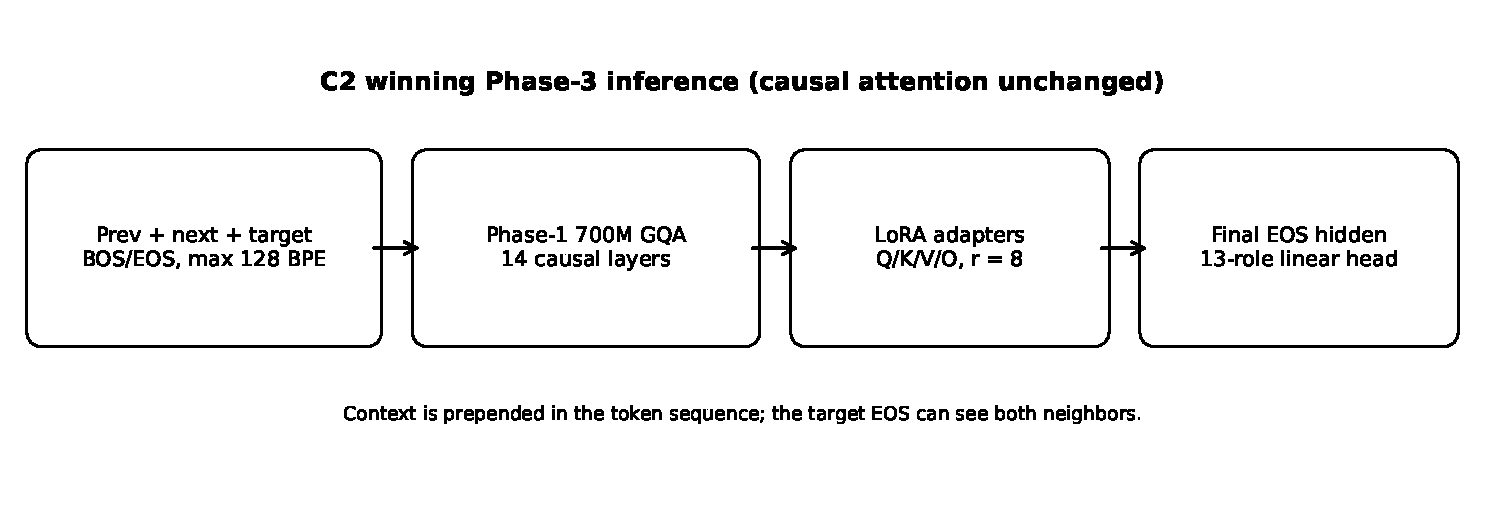
\includegraphics[width=.96\linewidth]{figures/phase3/p3_c2_architecture.pdf}
\caption{Actual C2 winning pipeline. Neighboring sentences are placed before the target under an unchanged causal 14-block Efficient GQA backbone; rank-8 LoRA adapters modify attention projections, and the final target EOS hidden state feeds a 13-class head. This is a schematic of executed inference, not a separately trained document encoder.}
\label{fig:p3-c2-architecture}
\end{figure}

\subsection{Adaptation methods and supervised optimization}
\label{sec:p3-methods}
The 14-block Phase-1 Efficient GQA model (768 hidden, 12 query heads, four KV heads, RoPE, RMSNorm and SwiGLU) was the principal backbone. Phase 3 used both the preserved 100M-token milestone and the continuation to approximately 700M consumed pretraining tokens. The four-architecture screening additionally used the original decoder-only, encoder--decoder and Prefix-LM backbones.

For frozen-base \emph{LoRA}, each selected attention projection received an additive rank-$r$ update,
\begin{equation}\label{eq:p3-lora}
 W' x=W_0 x+\frac{\alpha}{r}BAx,
\end{equation}
with $r=8$, $\alpha=16$ and adapter dropout 0.05. \emph{LoRMA+} used a different, multiplicative \emph{output-side} transformation of a base projection,
\begin{equation}\label{eq:p3-lorma}
 W' x=\left(I+\frac{\alpha}{r}BA\right)W_0x,
\end{equation}
initialized to the identity by setting $B=0$. All GQA attention projection biases are absent in the original architecture. \emph{IA$^3$} learned output scaling vectors for key/value projections and input scaling for the SwiGLU down projection; it did not update full projection matrices. \emph{Prefix tuning} learned 16 virtual key/value vectors per attention layer, visible to every real token while retaining causal real-token attention. The full-fine-tuning comparison updated all pretrained GQA parameters and the head. These were genuine changes of adaptation mechanism, not rank or learning-rate sweeps.

All main configurations used three-epoch budgets, AdamW with weight decay 0.01, batch size eight, two microbatches per optimizer update, gradient clipping to 1, a 5\% warmup followed by cosine decay, and development Macro-F1 checkpoint selection. Frozen-backbone adapter runs used learning rate $1.5\times10^{-4}$; full and student fine-tuning used $3\times10^{-5}$. Where supported, inference and training used BF16 autocasting. Model/head checkpoints and resumable optimizer states were saved separately in Drive; most training variants used a checkpoint every 300 optimizer updates, and the architecture-screening stage saved every 250 training batches. The best saved epoch was selected on development Macro-F1 and used for test inference. The original notebook contains one run per main condition, not repeated-seed estimates; dev-set tuning risks optimism with just ten judgments.

\subsection{Study design and actual experiment chronology}
\label{sec:p3-experiment-design}
\paragraph{Group A: four pretrained architectures and continued pretraining.}
A1--A4 held the LoRA method fixed while comparing standard causal decoder, encoder--decoder encoder, Prefix-LM and Efficient GQA (100M). A5 replaced only A4's foundation snapshot with the 700M GQA milestone. On development Macro-F1, the original GQA scored 0.3073 and the continued GQA 0.3291. The latter is a transfer improvement in this same-backbone comparison; the four-way architectural comparison still involves different objectives, dimensions, pooling and parameter counts.

\paragraph{Group B: adaptation mechanisms.}
On the 700M GQA, additive LoRA reached 0.3291 development F1; LoRMA+ reached 0.3171, IA$^3$ 0.2288, virtual prefix tuning 0.1983 and full fine-tuning 0.3330. Trainable parameter counts were respectively 583,437, 468,749, 45,837, 124,685 and 112,688,653. The full-fine-tuning gain over LoRA was only 0.0038 locally under these settings; without repeated seeds the experiment does not establish practical parity between the methods. The LoRMA+ official submission showed \method{Failed}, and the IA$^3$ submission showed \method{Preparing} in the supplied Codabench screenshot; both remain completed local training experiments and valid local prediction archives, but are not confirmed official evaluations.

\paragraph{Group C: context and structured decoding.}
C1 constructed \method{[BOS] [previous] [EOS] [target] [EOS]}. C2 constructed {\ttfamily\small [BOS] [previous] [EOS] [next] [EOS] [target] [EOS]}, omitting nonexistent neighbors at document boundaries. Context was budgeted inside the same 128-token limit; the target received at most about 65\% of the 126 content tokens, with remaining tokens divided between neighbors. Importantly, this is \emph{not} a bidirectional self-attention model: the GQA transformer remains causal, but the EOS summary of the final target can attend to tokens from both neighbors because both neighbors are placed earlier in the packed input. This design directly investigates the impact of legal discourse context.

C1 improved pooled dev Macro-F1 to 0.3424 and C2 to \textbf{0.3851}, versus 0.3291 without context. C3 instead estimated smoothed start-label and label-transition probabilities from training documents and performed document-wide Viterbi decoding on A5 emission log-probabilities. Transition strengths $\{0,.15,.30,.50,1,1.5,2\}$ were scored on development labels; 0.30 achieved 0.3527. This is a document-level \emph{structured postprocessor}, not a full-document neural text encoder or CRF-trained end-to-end. There was no hierarchical BiGRU, CRF or whole-judgment neural Transformer in the executed Phase-3 notebook.

\paragraph{Group D: joint versus domain-specific learning.}
D1 trained only CL judgments and D2 trained only IT judgments, evaluating each on both development domains. D1 achieved pooled 0.2215; D2 0.3020. Both lagged the joint A5 baseline (0.3291), although training-set sizes differed, so data volume and specialization are confounded. D3 used CL specialist outputs on CL test cases and IT specialist outputs on IT cases. This inference-only hybrid scored 0.3957 on the official hidden test, but the notebook did not record an independent development Macro-F1 for this hybrid; none is inferred here.

\paragraph{Group E: mandatory teacher--student knowledge distillation.}
The teacher was selected by development F1 among A5 and Group B, resulting in the fully fine-tuned GQA B4 at 0.3330. Both smaller students retained six layers $\{0,2,4,6,8,11\}$ from the original Phase-1 pretrained 12-layer decoder-only architecture, with 68,097,805 total parameters. E1 was trained using only hard labels. E2 used both ground truth and cached teacher-logit distributions:
\begin{equation}\label{eq:p3-kd}
 \mathcal L_{\rm KD}=\tfrac12\mathcal L_{\rm CE}+\tfrac12\, T^2 D_{\rm KL}\left(p_{\rm teacher}^{(T)}\Vert p_{\rm student}^{(T)}\right),\qquad T=2.
\end{equation}
E1 reached 0.3234 and E2 reached 0.3200 on development; corresponding official Macro-F1 scores were 0.3679 and 0.3638. Distillation therefore \emph{did not improve} predictive F1 in this controlled student comparison, although the smaller distilled student achieved about 3.69 times the teacher's measured sentence throughput (3,823 versus 1,035 sentences/s on the same fixed test subset). That benchmark measured throughput but did not isolate GPU memory: both models were resident simultaneously, so the reported peak GPU values are not reliable evidence of model-by-model peak-memory savings.

\paragraph{Group F: class-weighted loss.}
F1 used inverse-square-root class weights computed strictly from the training labels and clipped to $[0.2,5.0]$. It improved development Macro-F1 from A5's 0.3291 to 0.3459. Codabench displayed a numeric 0.3703 but also the \method{Failed} status; this cannot be counted as a confirmed official result without the failure details. It is nonetheless a meaningful local experiment.

\begin{figure}[htbp]\centering
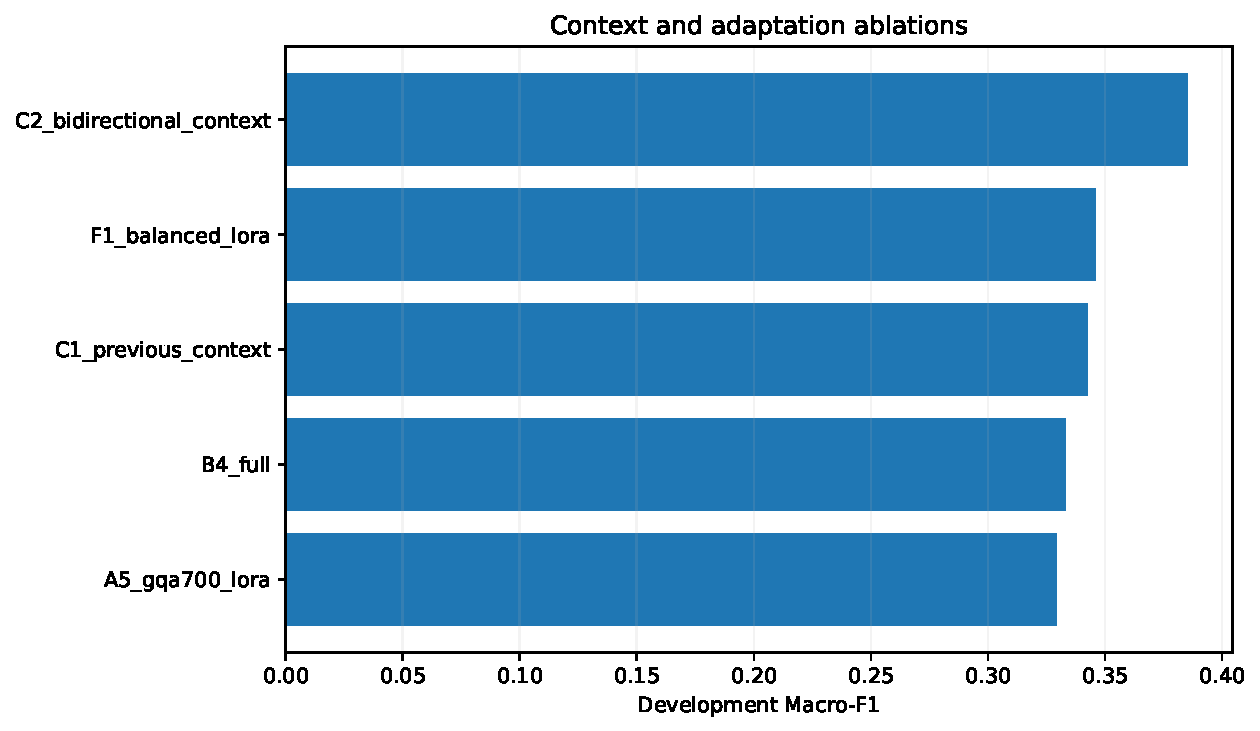
\includegraphics[width=.86\linewidth]{figures/phase3/p3_context_ablation.pdf}
\caption{Selected single-run development Macro-F1 results. The gain from C2 is measured against a shared 700M-GQA LoRA baseline with the same 128-token input budget; full-context performance was not evaluated through a separate hierarchical model.}
\label{fig:p3-context}
\end{figure}

\begin{figure}[htbp]\centering
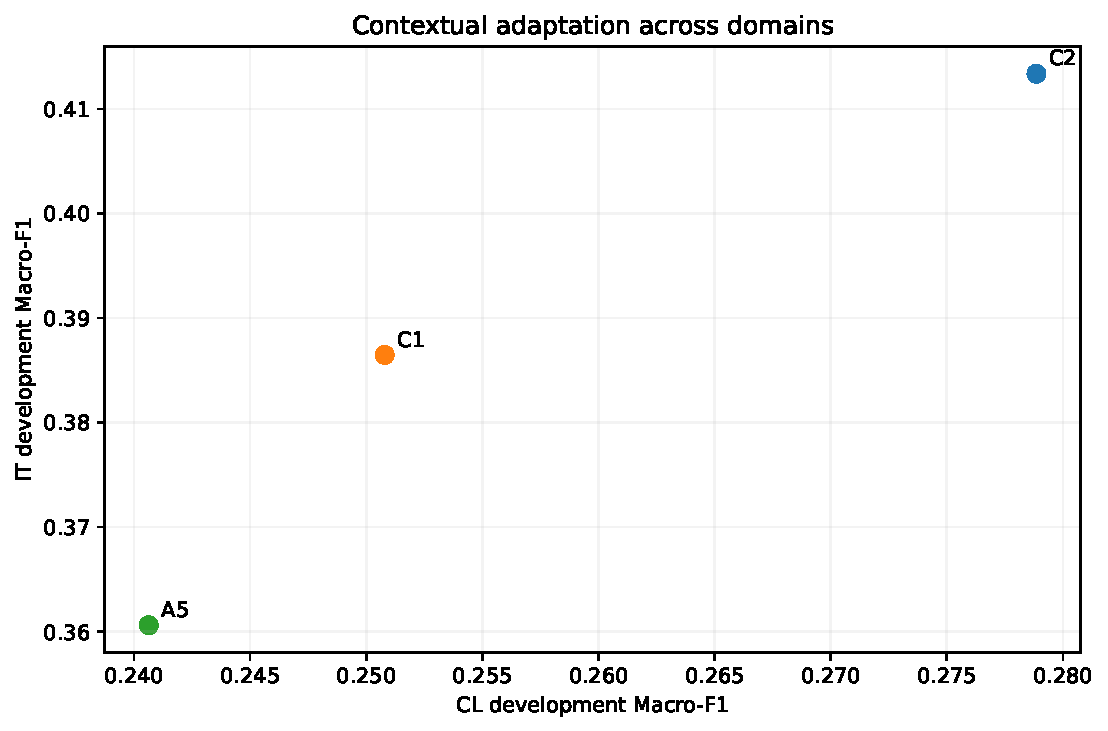
\includegraphics[width=.79\linewidth]{figures/phase3/p3_domain_comparison.pdf}
\caption{Development Macro-F1 by domain for baseline and local-context GQA. The official primary metric is pooled Macro-F1, not the arithmetic mean of the two domain scores.}
\label{fig:p3-domains}
\end{figure}

\subsection{Complete local and official results}
\label{sec:p3-results}
The notebook trained 16 independent classifier configurations. Two further candidate submissions were produced by postprocessing or combining trained outputs (C3 and D3), yielding 18 test archives. A local audit verified 10 required test-document IDs, 2,197 label predictions and exact allowed label names in every ZIP; this is a \emph{format and integrity} result, not proof that Codabench evaluated each one. The supplied screenshot shows 15 entries with a \method{Finished} score, one \method{Preparing}, and two \method{Failed}; two separate duplicate uploads for C2 and C3 were still \method{Submitting} at capture time.

\begin{longtable}{@{}r p{.44\linewidth} r r p{.14\linewidth}@{}}
\caption{Complete Phase-3 submission chronology. Development Macro-F1 is from the executed notebook and official Macro-F1 from the supplied Codabench screenshot. A numeric result in a Failed row is \emph{not} a confirmed completed evaluation. The D3 hybrid was not independently scored on development data.}\label{tab:p3-all}\\
\toprule
\# & Model or variant & Dev F1 & Official F1 & Status \\
\midrule\endfirsthead
\toprule
\# & Model or variant & Dev F1 & Official F1 & Status \\
\midrule\endhead
1 & A1\_\allowbreak decoder\_\allowbreak lora & 0.2934 & 0.3310 & Finished \\
2 & A2\_\allowbreak encdec\_\allowbreak lora & 0.1204 & 0.1361 & Finished \\
3 & A3\_\allowbreak prefix\_\allowbreak lora & 0.2350 & 0.2867 & Finished \\
4 & A4\_\allowbreak gqa100\_\allowbreak lora & 0.3073 & 0.3299 & Finished \\
5 & A5\_\allowbreak gqa700\_\allowbreak lora & 0.3291 & 0.3714 & Finished \\
6 & B1\_\allowbreak lorma\_\allowbreak plus & 0.3171 & -- & Failed \\
7 & B2\_\allowbreak ia3 & 0.2288 & -- & Preparing \\
8 & B3\_\allowbreak prefix & 0.1983 & 0.2379 & Finished \\
9 & B4\_\allowbreak full & 0.3330 & 0.4005 & Finished \\
10 & C1\_\allowbreak previous\_\allowbreak context & 0.3424 & 0.3976 & Finished \\
11 & \textbf{C2\_\allowbreak bidirectional\_\allowbreak context} & 0.3851 & \textbf{0.4249} & Finished \\
12 & C3\_\allowbreak document\_\allowbreak viterbi & 0.3527 & 0.3791 & Finished \\
13 & D1\_\allowbreak CL\_\allowbreak only & 0.2215 & 0.2586 & Finished \\
14 & D2\_\allowbreak IT\_\allowbreak only & 0.3020 & 0.3710 & Finished \\
15 & D3\_\allowbreak domain\_\allowbreak specialist\_\allowbreak hybrid & -- & 0.3957 & Finished \\
16 & E1\_\allowbreak student\_\allowbreak supervised & 0.3234 & 0.3679 & Finished \\
17 & E2\_\allowbreak student\_\allowbreak distilled & 0.3200 & 0.3638 & Finished \\
18 & F1\_\allowbreak balanced\_\allowbreak lora & 0.3459 & 0.3703 & Failed \\
\bottomrule
\end{longtable}


\begin{figure}[htbp]\centering
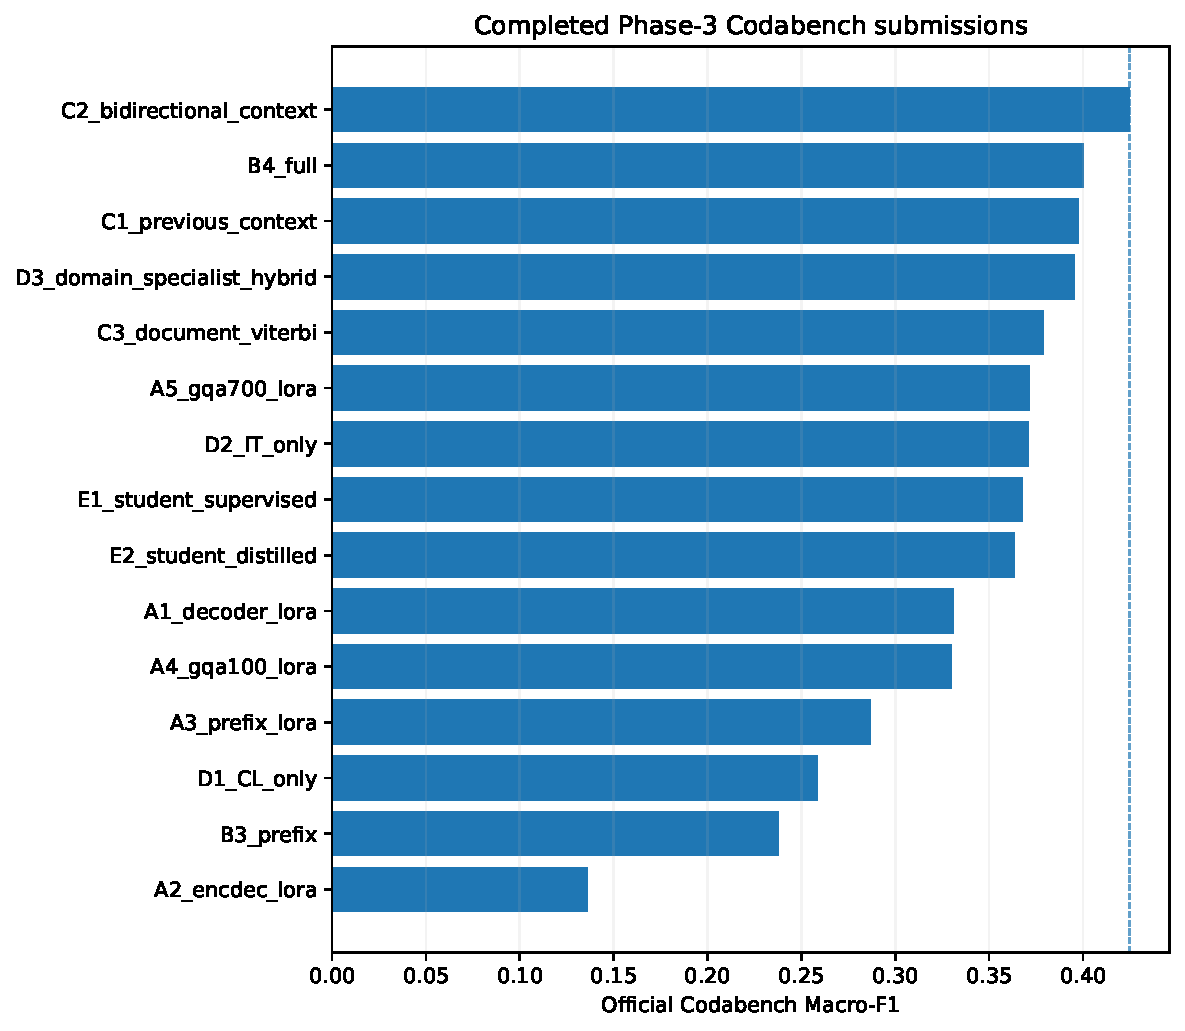
\includegraphics[width=.9\linewidth]{figures/phase3/p3_official_scores.pdf}
\caption{Official Phase-3 Macro-F1 for the 15 entries marked \method{Finished} in the supplied Codabench screenshot. Failed or pending rows are excluded even when a numeric value is visible.}
\label{fig:p3-official}
\end{figure}

\begin{figure}[htbp]\centering
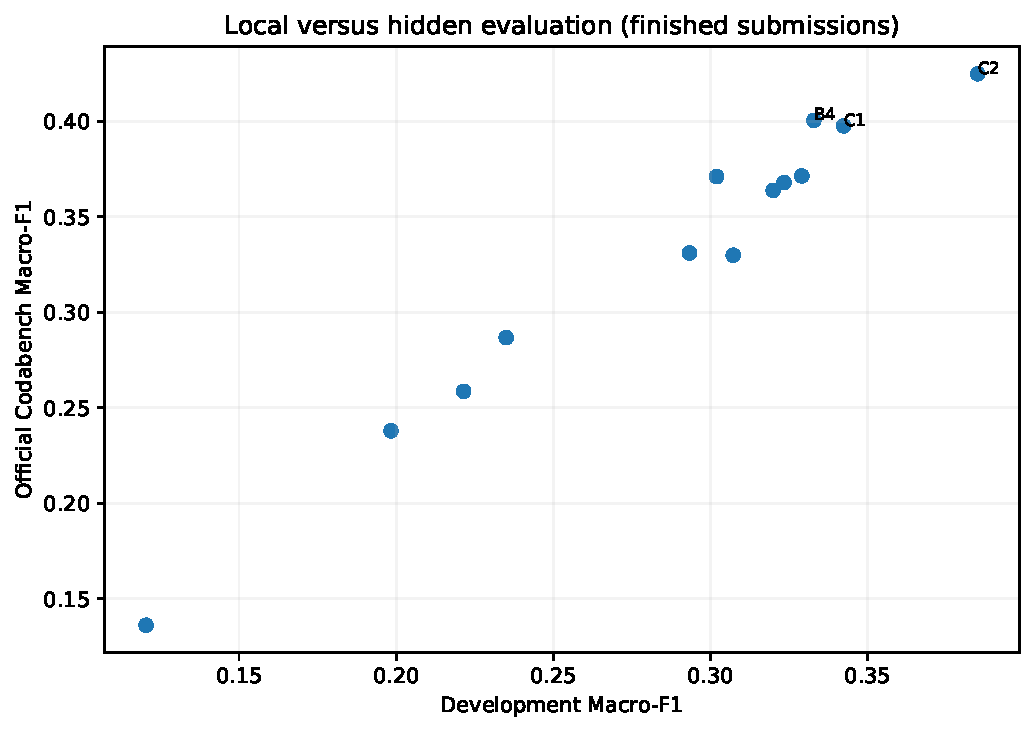
\includegraphics[width=.8\linewidth]{figures/phase3/p3_local_vs_official.pdf}
\caption{Notebook-selected local development F1 versus the official hidden-set primary metric for completed submissions with measured local scores. The plot makes the distinction between the two evaluation sources explicit.}
\label{fig:p3-local-official}
\end{figure}

The best confirmed official result is \textbf{C2 bidirectional-context GQA+LoRA, submission 989815, Macro-F1 0.4249}. By comparison, the same foundation and LoRA method without neighbors (A5) scored 0.3714, and the previous-sentence-only variant C1 scored 0.3976. The official C2--A5 gain is 0.0535 F1. C2 likewise led the local development analysis (0.3851), with the domain-wise development scores 0.2789 CL and 0.4134 IT. The official winner is selected by the private primary metric, not local training loss or larger trainable parameter count. We have no evidence of a numeric leaderboard rank and therefore report none.

\subsection{Error analysis and limitations}
\label{sec:p3-errors}
\begin{figure}[htbp]\centering
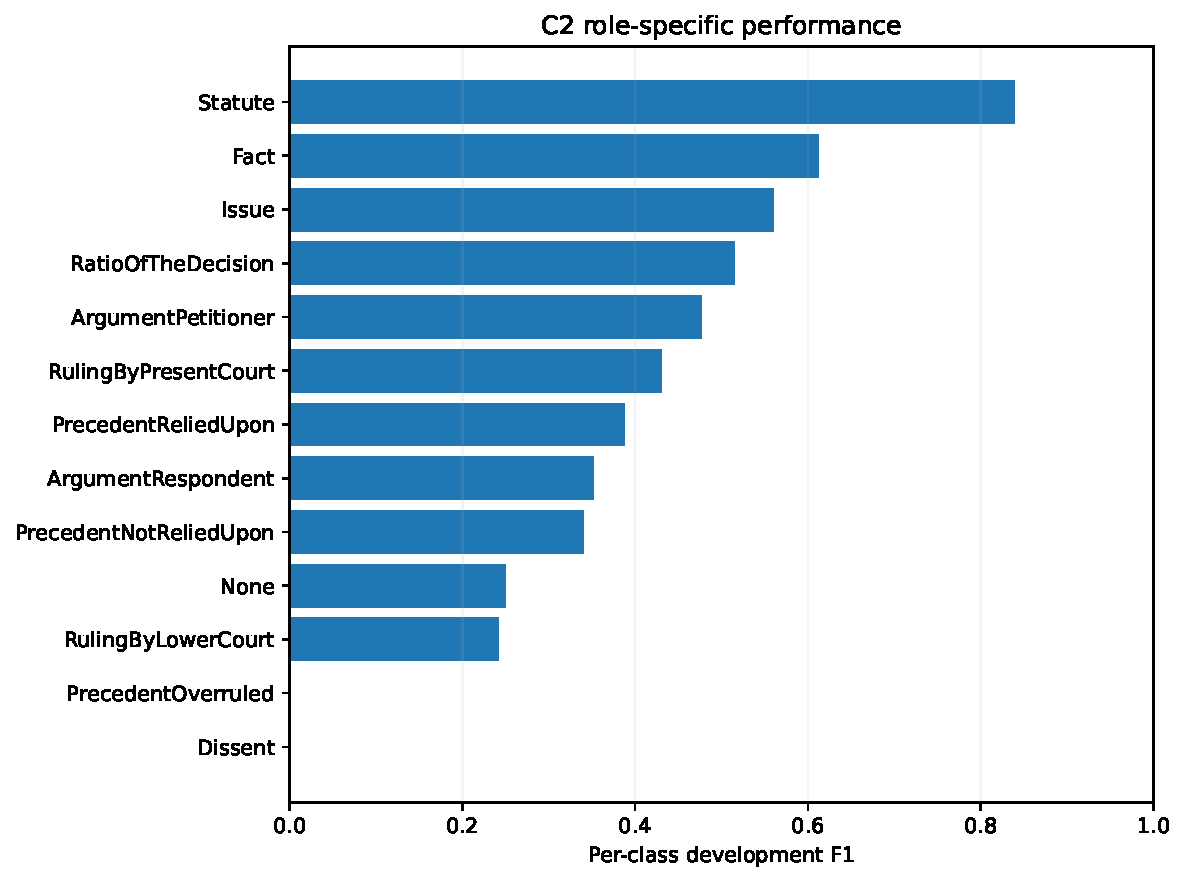
\includegraphics[width=.85\linewidth]{figures/phase3/p3_per_class_f1.pdf}
\caption{C2 development F1 for all 13 labels. The two classes absent from both development domains are scored zero by convention rather than treated as measured negative generalization cases.}
\label{fig:p3-classes}
\end{figure}

C2 produced development F1 0.839 for \method{Statute}, 0.613 for \method{Fact}, 0.560 for \method{Issue} (just 15 examples), 0.515 for \method{Ratio\allowbreak Of\allowbreak The\allowbreak Decision}, 0.352 for \method{Argument\allowbreak Respondent}, 0.242 for \method{Ruling\allowbreak By\allowbreak Lower\allowbreak Court}, and 0.250 for \method{None}. The strongest confusion in the saved error table was \method{Argument\allowbreak Petitioner} $\to$ \method{Ratio\allowbreak Of\allowbreak The\allowbreak Decision} (88 sentences), followed by \method{Precedent\allowbreak Relied\allowbreak Upon} $\to$ \method{Ratio\allowbreak Of\allowbreak The\allowbreak Decision} (81), \method{Fact} $\to$ \method{Ratio\allowbreak Of\allowbreak The\allowbreak Decision} (75) and \method{Argument\allowbreak Respondent} $\to$ \method{Ratio\allowbreak Of\allowbreak The\allowbreak Decision} (67). Other confusions included petitioner versus respondent arguments (46 in the petitioner-to-respondent direction and 60 in reverse) and lower-court ruling versus present-case reasoning (38 to \method{Ratio\allowbreak Of\allowbreak The\allowbreak Decision}). This pattern is consistent with difficulty separating reported legal positions from judicial reasoning, but it cannot prove the cause of any individual error without a contextual annotation audit.

The study is constrained by ten development judgments, uneven class support, one seed per central experiment and early stopping using the same small development set. Some comparisons change multiple factors: A1--A4 differ in pretraining objectives and pooling, and single-domain training changes both domain focus and the amount of available supervision. The 128-token cap and the 65\% target allocation in contextual runs truncate long sentences. There is no calibration or human expert review of ambiguous legal roles, no cross-domain held-out bootstrap interval, no direct paper-level claim of legal reasoning competence, and no independent validation of the official hidden labels. These limitations should be considered whenever interpreting differences of only a few F1 thousandths.

\subsection{Reproduction and winning-model handoff}
The clean research code is organized under \path{code/phase3/} and uses the existing \path{code/phase1/models.py} foundation definitions. It provides strict official JSON parsing, the original BPE token IDs, all adaptation methods, context building, native 13-class evaluation, resume-aware training, Viterbi decoding, hybrid composition, and strict ZIP validation. Local numeric evidence is retained in \path{code/phase3/experiments/}; the seven vector plots are regenerated from this evidence by \path{code/phase3/analysis/figures.py}. The best-model-only package is separate: it contains the exact GQA backbone, C2 attention LoRA, context encoding and inference routine, but not the research-only variants. Neither artifact includes pretrained weights, data or credentials.

The winning inference requires the preserved Phase-1 \path{best_up_to_700M.pt}, the Phase-3 \path{C2_bidirectional_context/best.pt} adapter/head state, and the original \path{legal_bpe_32k.json}. Validation of the archived original large backbone/adapter pair with regenerated bitwise-equivalent predictions remains pending where large remote checkpoint transfers are unavailable. Syntax tests, offline model smoke tests and format tests are valuable but cannot substitute for that final replay. The official hidden-test labels are not available and are not reconstructed.

\subsection{Conclusions and next research questions}
The Phase-3 study shows that compact, internally pretrained legal models are trainable for sentence-level rhetorical classification; the best measured improvement arose from \emph{neighboring-sentence context}, rather than a more expensive full fine-tune or a larger standalone head. Extended Phase-1 pretraining helped downstream local classification even though it did not improve Phase-1 hidden continuation BERTScore, illustrating task-dependent checkpoint value. Domain-only training was not competitive under the data available, and model compression improved measured throughput but did not improve F1 under this distillation objective. Further scientifically useful experiments would compare a hierarchical document encoder with the current causal context packing, apply document-level bootstrap intervals and multiple seeds, test calibrated rare-role handling, and isolate truncation effects on long judgments. None of these extensions is misrepresented as a completed Phase-3 experiment.
